\documentclass{sigchi}

% Use this section to set the ACM copyright statement (e.g. for
% preprints).  Consult the conference website for the camera-ready
% copyright statement.

% Copyright
% \CopyrightYear{2016}
% %\setcopyright{acmcopyright}
% \setcopyright{acmlicensed}
% %\setcopyright{rightsretained}
% %\setcopyright{usgov}
% %\setcopyright{usgovmixed}
% %\setcopyright{cagov}
% %\setcopyright{cagovmixed}
% % DOI
% \doi{http://dx.doi.org/10.475/123_4}
% % ISBN
% \isbn{123-4567-24-567/08/06}
% %Conference
% \conferenceinfo{CHI'16,}{May 07--12, 2016, San Jose, CA, USA}
% %Price
% \acmPrice{\$15.00}

% Use this command to override the default ACM copyright statement
% (e.g. for preprints).  Consult the conference website for the
% camera-ready copyright statement.

%% HOW TO OVERRIDE THE DEFAULT COPYRIGHT STRIP --
%% Please note you need to make sure the copy for your specific
%% license is used here!
% \toappear{
% Permission to make digital or hard copies of all or part of this work
% for personal or classroom use is granted without fee provided that
% copies are not made or distributed for profit or commercial advantage
% and that copies bear this notice and the full citation on the first
% page. Copyrights for components of this work owned by others than ACM
% must be honored. Abstracting with credit is permitted. To copy
% otherwise, or republish, to post on servers or to redistribute to
% lists, requires prior specific permission and/or a fee. Request
% permissions from \href{mailto:Permissions@acm.org}{Permissions@acm.org}. \\
% \emph{CHI '16},  May 07--12, 2016, San Jose, CA, USA \\
% ACM xxx-x-xxxx-xxxx-x/xx/xx\ldots \$15.00 \\
% DOI: \url{http://dx.doi.org/xx.xxxx/xxxxxxx.xxxxxxx}
% }

% Arabic page numbers for submission.  Remove this line to eliminate
% page numbers for the camera ready copy
% \pagenumbering{arabic}

% Load basic packages
\usepackage{balance}       % to better equalize the last page
\usepackage{graphics}      % for EPS, load graphicx instead
\usepackage[T1]{fontenc}   % for umlauts and other diaeresis
\usepackage{txfonts}
\usepackage[utf8]{inputenc}
\usepackage{mathptmx}
\usepackage[pdflang={en-US},pdftex]{hyperref}
\usepackage{color}
\usepackage{booktabs}
\usepackage{textcomp}

% Some optional stuff you might like/need.
\usepackage{microtype}        % Improved Tracking and Kerning
% \usepackage[all]{hypcap}    % Fixes bug in hyperref caption linking
\usepackage{ccicons}          % Cite your images correctly!
% \usepackage[utf8]{inputenc} % for a UTF8 editor only

% If you want to use todo notes, marginpars etc. during creation of
% your draft document, you have to enable the "chi_draft" option for
% the document class. To do this, change the very first line to:
% "\documentclass[chi_draft]{sigchi}". You can then place todo notes
% by using the "\todo{...}"  command. Make sure to disable the draft
% option again before submitting your final document.
\usepackage{todonotes}

% Paper metadata (use plain text, for PDF inclusion and later
% re-using, if desired).  Use \emtpyauthor when submitting for review
% so you remain anonymous.
\def\plaintitle{Body-worn controllers and E-Textiles - Interaction and social acceptability}
\def\plainauthor{First Author, Second Author, Third Author,
  Fourth Author}
\def\emptyauthor{}
\def\plainkeywords{Authors' choice; of terms; separated; by
  semicolons; include commas, within terms only; required.}
\def\plaingeneralterms{Documentation, Standardization}

% llt: Define a global style for URLs, rather that the default one
\makeatletter
\def\url@leostyle{%
  \@ifundefined{selectfont}{
    \def\UrlFont{\sf}
  }{
    \def\UrlFont{\small\bf\ttfamily}
  }}
\makeatother
\urlstyle{leo}
%NO DOI
\doi{-}
%NO isbn
\isbn{-}
% To make various LaTeX processors do the right thing with page size.
\def\pprw{8.5in}
\def\pprh{11in}
\special{papersize=\pprw,\pprh}
\setlength{\paperwidth}{\pprw}
\setlength{\paperheight}{\pprh}
\setlength{\pdfpagewidth}{\pprw}
\setlength{\pdfpageheight}{\pprh}

% Make sure hyperref comes last of your loaded packages, to give it a
% fighting chance of not being over-written, since its job is to
% redefine many LaTeX commands.
\definecolor{linkColor}{RGB}{6,125,233}
\hypersetup{%
  pdftitle={\plaintitle},
% Use \plainauthor for final version.
%  pdfauthor={\plainauthor},
  pdfauthor={\emptyauthor},
  pdfkeywords={\plainkeywords},
  pdfdisplaydoctitle=true, % For Accessibility
  bookmarksnumbered,
  pdfstartview={FitH},
  colorlinks,
  citecolor=black,
  filecolor=black,
  linkcolor=black,
  urlcolor=linkColor,
  breaklinks=true,
  hypertexnames=false
}

% create a shortcut to typeset table headings
% \newcommand\tabhead[1]{\small\textbf{#1}}

% End of preamble. Here it comes the document.
\begin{document}
\title{\plaintitle}
\numberofauthors{4}
\author{%
  \alignauthor{Leave Authors Anonymous\\
    \affaddr{for Submission}\\
    \affaddr{City, Country}\\
    \email{e-mail address}}\\
  \alignauthor{Leave Authors Anonymous\\
    \affaddr{for Submission}\\
    \affaddr{City, Country}\\
    \email{e-mail address}}\\
  \alignauthor{Leave Authors Anonymous\\
    \affaddr{for Submission}\\
    \affaddr{City, Country}\\
    \email{e-mail address}}\\
  \alignauthor{Leave Authors Anonymous\\
    \affaddr{for Submission}\\
    \affaddr{City, Country}\\
    \email{e-mail address}}\\
}

\maketitle

\begin{abstract}
  Smart Textiles and body worn controller (Wearables) have been analyzed, mostly individually, using different technologies and on different aspects. Although there were some tests concerning everyday life, they are not used very often in this situation life for several reasons. This paper aims to show some of them and analyze, instead, the opportunities that  may lead to a better development and improve the feeling that a user has when interacting in an uncommon way with a device. One of the main threats that this paper discuss will be the reasons for social unacceptability, methods to review social acceptability and possible solutions for the problems concerning the usage of Wearables in public minding also technology-related tradeoffs.
  To illustrate the issues different Wearables are going to be presented - specifically concentrating on the social aspects of the devices. Finally this paper discusses further development of social acceptability of Wearables in the future.
\end{abstract}
% \category{H.5.m.}{Information Interfaces and Presentation
%   (e.g. HCI)}{Miscellaneous} \category{See
%   \url{http://acm.org/about/class/1998/} for the full list of ACM
%   classifiers. This section is required.}{}{}
%
% \keywords{\plainkeywords}
%
% \section{Introduction} \label{test:intro}
%
% Here there's the intro.
% \\ \textbf{Bold text} is done with
% \begin{verbatim}
%   \textbf{Bold text}
% \end{verbatim}
% \emph{emphatized text} is done with
% \begin{verbatim}
%   \emph{emphatized text}
% \end{verbatim}
% New line is made with double backslash
% \begin{verbatim}
%   line \\ another line
% \end{verbatim}
% \subsection{A subsection}
% Text of the subsection is shown here.
% \subsubsection{This is a subsubsection}
% We should not go further in sub sectioning, so we shall not use \textit{paragraph} and \textit{subparagraph}
% % References must be the same font size as other body text.
\section{Introduction}
%
% quick overview over the topic. Philipp already mentioned that his abstract might be a good starting point.
% Also we should give an introduction on the respective parts of the paper and give reason for the research we did (why is social acceptability an issue…)

Touch gestures are a form of interaction that is used by almost everyone daily in our society. Whether Smartphone, Tablet or Smartwatch - many mobile devices are nowadays controlled by this input technique to master different tasks. High demands are directly related to the fast and intuitive use of these devices. The combination of different electronic devices can help achieving these requirements in a new measure. For example, smart watches are already used to control mobile phones or various home electronics (e.g. controlling lamps). The development of innovative input devices, which can be integrated into clothing or even applied to the user's skin, offers the potential to communicate with electronic devices in completely new ways and make interaction even more intuitive. In this paper we especially focus on touch input devices that are attached to the user's skin or are integrated into clothing and can be used to control different electronic devices.
Because these technologies create new and unusual forms of interaction, we will also look on third-party perceptions of a user’s interactions with a wearable E-textile interface. Social conventions play an important role in the development of these new forms of interaction. The willingness make a gesture depends largely on how appropriate these interaction look and feel in public. \cite{touch-wrist} The usability of these technologies must also be examined: to support the user as efficiently, effectively and satisfactorily as possible, the designers must consider the interaction with the system in addition to the placement of this body-worn controllers.

\section{Showcase of technology examples}
%
% Maybe first a definition of body-worn controllers and a not, that we want to concentrate on Touch-Input.
% I think it is a good idea to pick a few examples which were mentioned in the papers and discuss them briefly.
% For the first part (just the showcase) it is sufficient to just write down the basic technology (with Source): So what it is? How does is work (very briefly)? What it is used for?
% We can get more into detail in the pros/cons section below
The body worn controllers\footnote{input sources made by joining small electric devices with everyday worn clothing} %footnote
allows to have bigger controlling surfaces ready to be used without needing to take out the main device. Moreover, these controllers allow to express input gestures, which are comparable to everyday gestures. Therefore allowing the user to express emotions while using the device. If on a touchscreen the feedback of the input is based only on vibration and visual input. With body-worn controllers the input surface is set over the skin, which allows a direct feedback to the user, that includes the emotion put into performing a gesture. An example made by Wiegel et Al. %in More Than Touch
\cite[p.185]{more-touch} is “Uncomfortable interactions were chosen for actions that are very important and not reversible”, which shows how the gesture chosen to perform an action were related to the consequence that this action may lead to.

%Belt feels a bit off in this position. We should group it in one of the other sections (probably eTextiles) or add a header just for itself, as an example for a body worn controller.
%agree - Andrea

Augmented Reality related research is still trying to optimise the input, which interacts with the shown interface, so that it could potentially capitalize on the natural and unobtrusive ways you interact with Wearables.
“Belt” \cite{belt} is an body-worn controller specifically build to interact with Augmented Reality applications. As the name suggests the device is worn around the hip, like a regular belt which is touch-sensitive and can differentiate between simple gestures and locate the position of the touch-input \cite[p. 2136]{belt}.%([8] Page 2136).
One of the main use cases of the device are spatial mapped shortcuts to open apps, like a virtual wallet. \cite{belt}

\section{Body-worn sensors}
% also true for iSkin
A current approach deals with the placement of multi-touch sensors directly on the skin. Because the human body surface is irregularly curved and deformable, the system must be particularly flexible and adaptable to fit the skin. This is a special requirement for the design of the sensors as it needs to satisfy the comfort of the user wearing it, who should not feel the fact that he is wearing a sensor. \cite{ulbrich2,iSkin}%[2, 3]

Furthermore, the human body has capacitive effects, which must be correctly shielded from an input sensor to ensure reliable touch detection. This places special demands on the technology's material: it must both be insulated by the conductive sweat produced by the skin, but it has to let the same sweat flow outside, to avoid the user to feel uncomfortable due to the impossibility of the the skin to dissipate the heat in that area. \cite{ulbrich2} %[2]
To master these challenges, the researchers of “Multi-Touch Skin” \cite{ulbrich2} studied various materials and manufacturing processes. As a result of this research work, a multi-touch sensor was developed, which can be applied directly to the user's skin in the form of a thin layer and capable of adapting flexibly to the different body shapes. To counteract the capacitive properties of the human body, the prototype consists of three layers, the transmitting, receiving and shielding layer. The individual layers are produced using a standard printer. Silver ink was used here because silver is a particularly effective electrical conductor and so is perfectly qualified to produce the sensor units. Furthermore, this method is well suited to produce multi-touch sensors in different sizes and therefore to test them on different body regions. \cite{ulbrich2}
A small multi-touch sensor behind the ear could be used to manipulate an audio device. For example, the user could adjust the volume by stroking the sensor or pause playback with a simple click. A wristband sized sensor could be used to control interactive lamps. Users could place two fingers around the wrist and rotate them to change the color of a light bulb or adjust the brightness of a lamp using swipe gestures. \cite{ulbrich2}

Another solution is presented by iSkin \cite{iSkin}, where a different material is used to allow input to be sensed. The polydimethylsiloxane (PDMS), the silicon-based material used, is “fully transparent, elastic, and a highly biocompatible material. [...] Therefore it is widely used on or in the human body, for example in body implants.” \cite[p. 2994]{iSkin} PDMS is non-conductive, but adding carbon to it lead to cPDMS, which can create a conductive surface. This allows to create gray sensible surfaces with specific drawn theme on it, that can immediately let the user know what to press for an action, but it doesn’t allow gestures to be performed on as the principle on which it’s build is an RC charge-discharge time evaluation of the sensible surface \footnote{An RC electronic circuit has a typical charge-discharge time constant $\tau$ which is given by the product $R \cdot C$. when pressure is applied, capacitance changes as the distance between the two surfaces it’s reduced. When a different charging time is sensed, the pressure is identified.}.

\section{E-Textiles}
E-textiles, the contraction of electronic textiles, are input devices fitted or integrated into the fabric of a user's clothing. These surfaces allow the user to interact with various electronic devices in his environment, as they integrates both the sensing surface, which takes the physical input like touch, grab or fingering,  and a control unit, which elaborate the input and send it to a controlled device. This means that usually an E-textile is only an input surface, which implies the necessity for the surface itself not to be rigid in order to let the skin act as a direct feedback for the user.
An example for E-Textiles is “Pinstripe” a project by the University Aachen\cite{pinstripe}. This technology is directly integrated in clothing by conductive threads. The threads measure folds, which are created by pinching the fabric with thumb and index finger. When the fold is rolled across the fabric the rolling gesture accompanied by the diameter of the fold acts as an input (smaller folds represent finer inputs). Those inputs can be used for example to manipulate the volume of a music player. %\cite{pinstripe}%[6]
Another E-textile is the ``Jogwheel'', which was developed as part of the paper ``Don't Mind Me Touching My Wrist[...]'' \cite{touch-wrist} to investigate the social acceptance of on-body technology. The Jogwheel is visually comparable to a fabric patch and is made of conductive yarn. A tactile surface structure should guide the user's fingers, which simplifies eye-free interaction. The developers describe the size of the Jogwheel as twice the size of the iPod click wheel. This size should allow high precision in use and several types of one-handed gestures.
Figure \ref{fig:1} show the Jogwheel and two ways of interaction with them. The E-Textil can be placed anywhere on the user's clothing for controlling electronic devices. \cite{touch-wrist}

\begin{figure}
  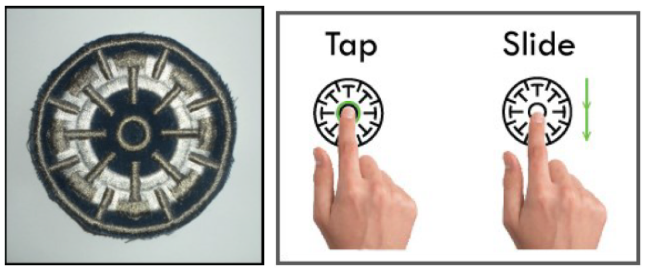
\includegraphics[width=\columnwidth]{jogwheel.png}
  \caption{\emph{Jogwheel} as presented in \protect\cite{touch-wrist}}
  \label{fig:1}
\end{figure}
%
%
% here we can add everything to e-Textiles
Another type of E-textile is the one presented by SmartSleeve \cite{smart-sleeve}, where the fabric is an input surface made alternating conductive and insulating textile bands. Then another pressure-sensible fabric is set under the first one, beneath which there’s another fabric alternating conductive and non-conductive bands  orthogonal to the top layer. This allows to touch and register both the position and the intensity with a matrix representation. The sensor density is 1.66 sensors per square inch, which allows for a discrete sensor density. However, as the system is working with the short-circuit principle and the wires are not insulated, skin moisture can lead to false position sensing. To avoid that, the authors have put SmartSleeve over a long-sleeved running shirt. This solution, though, becomes unsuitable in summer for obvious reasons. %maybe better written
%
Project Jaquard \cite{jacquard}, instead, utilizes a capacitive system where the fabric is one layer textile where some of the wires in the weft and warp are electrical wires. As the touch sensing is made with capacitance measure, this system is not vulnerable to errors due to the skin moisture. Different materials have been investigated to create the electrical wires, both for simplicity over the creation of the fabric and the necessity of flexibility needed for comfort. The material chosen is copper because it has similar properties to cotton, silk and wool when the wire diameter is 50µm.
%
% \subsection{SimpleSkin: Towards Multipurpose Smart Garments}
The Simple Skin \cite{simpleskin} is an example of modular smart textile garment, created for commercially viable multi-purpose garments. It combines multiple sensing modalities, namely capacitive sensing for head and wrist movement , resistive sensing for arm movement \cite{vogel4}, bio-impedance sensing for heart rate and optional smartphone interaction. This placement is intended to detect the angles of the joints to analyse posture, monitor vital signs and offer input on the socially accepted region of the lower arm with the wrist sensor. Finally, the smartphone grants the options of a regular input device or a supportive device to supply the user with  information. Its modular design offers a separation of the concerns for sensing, acquisition hardware, processing and software, allowing for the use of various combinations of different technologies on the same garment and enables modifications of the underlying fabric with detachable hardware. \cite{simpleskin}

\section{Advantages and disadvantages of body-worn controllers}
Body-worn controllers offer innovative solutions to a host of problems, facilitated by a combination of progressive miniaturization and sophistication of electrical components. Recent miniature controllers in the form of smart-watches and wristbands can complement larger devices by supplying information or substitute them as more limited but less power-consuming alternatives. \cite{motion-ui} Although Smartphones are undoubtedly the most ubiquitous form of small computing devices, improvements can be made: Mobile phones are large enough to offer extensive functionality and services, but their use can be distracting, due to the length of interactions, or even objectionable, in certain social settings. Phones are usually kept out of sight, retrieved when needed, then returned to their container or receptacle to conform to social etiquette. They also demand more concentration from the user, preventing effective use while moving or attempting to execute other tasks that require coordination. Smaller body-worn devices, for example in the form of wrist-worn contraptions, can be worn in an unremarkable and acceptable manner and remove the need for retrieval and concealment for their use. The design of new interfaces for these body-worn devices also allows for the development of more concise interaction, reducing access time to return to the previous task without interruption in a “micro-interaction” cycle.\footnote{Microinteractions: interactions with a device that take less than four seconds to initiate and complete.} \cite{microinteraction}
Yet for all the innovative concepts developed with these technologies, they have not reached the level of ubiquity of their handheld Smartphone counterparts.
This is in part due to inherent size restrictions for the sake of user convenience. Controllers are designed to be worn in a fashion conforming to conventional accessories, usually situated on the upper body for manual access. Any unnecessary bulk is trimmed to not encumber the user, especially in the case of distally attached gadgets. This comes at the cost of display sizes, resulting in diminutive screens operated by basic button controls, which can be unintuitive, or touch input, which is made difficult by ``fat-finger’’ issues\footnote{A fat-finger error is a human error caused by pressing the wrong key when using a computer to input data.} %footnote
with the limited size. Operating conventional graphical interfaces like the QWERTY keyboard on very small screens is not very practical: The input method requires precious screen space to display a touchscreen keyboard and precise positioning of the fingers tips to avoid input errors. \cite{vogel7} Research efforts are being made to remedy these problems in circumstances where screen enlargement would contradict concept goals or redesigning screen real estate\footnote{Screen real estate is the amount of space available on a display for an application to provide output. } %footnote
use would  be deemed ineffective. These efforts are directed towards introducing more naturalistic and expressive user interfaces for existing hardware as well as methods to influence gesture recognition by improving the goodness of input. \cite{motion-ui, vogel7} %[10, 11]



\section{Social acceptability of touch-based Wearables}
% In this part we should discuss the issues with social acceptability
% first in general
% second regarding the specific devices we presented in the showcase
% When developing body-worn controllers, two things have to be considered. On the one hand the body part where this technology is placed - on the other, the design of the technology so that the system adapts as well as possible to the selected body part. These two parameters are a basic requirement for the most user-friendly system. [Source: Don't Mind me Touching my wrist]. However, another parameter is crucial and will be discussed in more detail in this section - social acceptability.
When developing body-worn controllers, two things have to be considered. On the one hand the body part where this technology is placed - on the other, the design of the technology so that the system adapts as well as possible to the selected body part. These two parameters are a basic requirement for the most user-friendly system. \cite{touch-wrist} However, another parameter is crucial and will be discussed in more detail in this section - social acceptability.

Social acceptance includes the social competence and presentation in which people behave in such a way that they feel comfortable in society or do not embarrass themselves or draw attention to themselves. \cite{self-everyday} The use of portable technologies is therefore also subject to social conventions. The body-worn controllers listed in the previous sections are associated with new designs, new shapes and, above all, new interactions that might seem unfamiliar to third parties at first appearances.
An example of this is the Bluetooth headset from the early 2000s. At first, there was less acceptance in society because it looked as if the user was talking to himself. After a while, however, the Bluetooth headset became established in society. \cite{usable-gesture} The use of body-worn controllers could initially lead to similar effects and acceptance problems, for which reason possible application examples are presented below, evaluated and discussed with the aid of current studies.

The perception of technology use in public spaces can be different in every culture, because the standards of social behaviour vary in many countries. This also should be considered in the development of new interactive systems, which is why it also needs to be part of the research of social acceptance. Campbell et al. have shown in their study on the public use of mobile phones, that there are indeed differences in this field. For example, Campbell et al. discovered that in Japan the use of mobile phones in buses or sidewalks is less accepted by society than in a restaurant. In many other cultures, this is rather the opposite. \cite{mobile-phones} These results lead to the conclusion that there are also cultural differences in perception when interacting with body-worn controllers which need to be explored.

Social acceptance includes various factors, which is why different methods are used to evaluate them. A handful of these methods will be mentioned and discussed in the next section.

\subsection{Methods to review social acceptability}
%
% During my research I stumbled upon various methods to review the social acceptability of wearables (testing devices in public, testing devices in labs, testing with functional devices, testing with dummies, interviews which were more like a conversation, interviews with a simple likert scale (1..5) … the list goes on)
% We should discuss these techniques - what are advantages, disadvantages? What methods are practical / necessary?

Since social acceptability is a major issue when it comes to the adaptation of new technology there is also the need to measure it appropriately. Different researches have different approaches to review the social acceptability of their respective research. \cite{touch-wrist}

\section{Testing - Demonstrating Technology}

\subsection{Testing with dummy (without working technology)}
% Belt (public), Usable Gestures, More Than Touch
One of the first possible ways to study and discuss both comfort and easiness  to interact with clothing as an input, is to interview people about what they would do to enact some commands on their skin. This is the main principle adopted by the Paper ``More Than Touch’’ \cite[p. 181]{more-touch}, where the authors say: ``This allowed us to observe participants’ unrevised behavior, free of the restrictions of current hardware. This method prove helpful in previous work for deriving implications for future hardware and system designs to accommodate this user behavior.’’
These research types allow to have a common ground, as they help defining areas where the touching is not possible, either because it’s a position not easily acceptable or because it’s not a social acceptable position. Testing usually is done in a laboratory, like with ``Usable Gestures’’ \cite{usable-gesture}, where the user feels less the social pressure given by the presence of many people. So this type of testing is quite useful when beginning the development of a technology, as it’s not related to the current hardware, but has some limitations both because it doesn’t consider the necessary tradeoffs that must be made to go from the idea of the device to the actual working device and because the laboratory itself doesn’t reflect the everyday situation that a person and a device will encounter on.

\subsection{Testing in private (lab situation)}
% Belt (working prototype), Pinstripe, Usable Gestures, More Than Touch, SmartSleeve
Tests in a lab offer special possibilities. On one side the subject is not distracted by other stimuli and is more focused on the presented topic (in this case gesture testing). On the other side researchers can verify more data recorded by the sensor, receive voice feedback by the testing subject, which can include what and why they’re doing, the mental model behind the specific gesture, while they’re performing it.
The first prototype shown is ``Belt'' \cite{belt}, here users had a visual feedback for the belt-interaction, which was Google Glass. The main result, common to all interactions, is that the area reachable to the dominant hand is preferred. In the Belt case, in particular, the area which had a higher number of shortcuts is the front of the belt on the side of the dominant hand, where users expressed the easiness and comfortability of interacting with a body-worn device. The second case-study taken into account by this paper is ``Pinstripe'' \cite{pinstripe} in which test subjects would perform gestures in three different contexts, which are sitting, standing still and walking, and for each of them they’ll try to perform a grabbing gesture in all the sixteen areas of their body defined by the authors. For each of them they expressed the easiness and the personal acceptance of doing that gesture in that context. The most important discovery, found out also by the papers \cite{social-comfort, belt,more-touch}, is that the preferred part of the body is the upper side of the body, both for accessibility, which relates to easiness, and the comfort related to the social acceptance.
Moreover, as shown by \cite{more-touch} the mind model related to the touchscreen UI influences mostly the types of gestures (i.e. pinch to zoom is transferred from the Smartphone to the textile surface)

\subsection{Testing in public}
% Belt (no working tech), Usable Gestures, Pinstripe
%
When transferring from the private laboratory environment to the public and social environment where the subject meets people who are looking to himself, some different aspects can be noticed: first of all, the area, that was shown as acceptable is reduced considerably and comprehend only the arm, the pocket area and the sternum \cite{pinstripe}. This can be related to ``More than Touch’’  \cite{more-touch} were people felt uncomfortable in areas where they’re not used to perform touch gestures. An example that we can make is the fact that in the pocket area is normally reached to get the Smartphone, the wallet or the keys. In case of the forearm, instead, a person may look at his watch multiple times a day. One remark made in ``Pinstripe’’ \cite{pinstripe}, in fact, was that even though the sternum had a high rating. Female testers were underlying that it would not be socially acceptable to interact in that area, so the areas where the input should be placed depends on cultural background, sex and personal attitude.
When it comes to testing technology in public the most important factor is the observer. In the research done by Rico et. al. \cite{usable-gesture} one observation was, that not only the location played an important role, when it came to performing unusual gestures, but also the amount of observers and the degree of acquaintance. So in order to review a technology, which should be used in public situations, one has to test it in public situations to accurately define the degree of social acceptability.
“Because we observed differences between the first and second trials, we would recommend completing at least two trials when evaluating for social acceptability because users will develop preferences and change their acceptance rates after multiple trials. Additionally, we suggest that such trials be completed in real world settings, rather than lab ones.” \cite[p. 9]{usable-gesture}%([5] page 9)

\subsection{Testing with device (working technology)}
% Belt (private), Pinstripe, Usable Gestures
When reviewing the social acceptability of a product and on a larger scale even the product itself at last it comes down to testing with the device itself. Tests with a dummy are inherently easy to set up and do not require costly prototypes. They can also yield interesting, insightful results, especially when it comes to reviewing the gestures and overall appearance. On the other hand there are some aspects you can only truly examine while testing with working technology. These aspects include for example the actual amount of distraction the user experiences while using the device. A survey participant might experience some minor distraction while practicing a gesture with a dummy and simultaneously talking to a person. When he now repeats the same gesture with working a working Augmented Reality Wearable he might encounter a stronger level of distraction due to the Augmented Reality Overlays which are shown to him.
To avoid insufficient dummy tests both techniques are often combined to create a time- and cost-efficient solution with satisfactory results.

\subsubsection{Demo video showing technology}
% Don’t mind Me, The Social Comfort, Usable Gestures
Demonstrating a demo video to participants that represents the usage of a technology in a public situation can be a good way to get feedback regarding social acceptance. The paper ``Don't Mind Me Touching My Wrist: [...]’’\cite{touch-wrist} deals with this issue and examines which cultural differences of perception can arise during interaction with an E-Textile. \cite{touch-wrist} The USA and South Korea were chosen as reference countries for this purpose. In order to investigate perception, the ``Jogwheel’’ was used, which we have already discussed above. The use case was the control of a mobile phone, to be exact, muting it after an incoming call, during a four eye conversation in an elevator. The scenario was simulated twice in each of the two countries - once the interaction with the Jogwheel was done by a woman and once by a man. This was recorded by camera and then the video was presented to the participants in an online-survey. This allows evaluation of the scenarios in public context. The video was shown to the participants once with a view from a distance (~1.2-1.5 meters) and once with a focus on the interaction (distance ~30-45 centimeters)). After the video, the participants were asked various questions about the interaction shown with the Jogwheel and its body placement. The questions were answered by using the Likert scale, given values and personal opinions of the participants. \cite{touch-wrist} In combination with an online survey, this test method offers the advantage of evaluating the scenarios in a public context. Furthermore, larger numbers of participants can be achieved through easier sharing of the videos/survey. \cite{touch-wrist}

\subsection{Interviews}
When conducting a research based on interviews the first approach is often to offer the subjects a multiple choice style answer sheet. This technique yields a few very obvious advantages. The results are very comparable and the answers are always very clear. The interviews are also faster - so a larger number of subjects can be interviewed in less time. One major disadvantage is that the answers are always represented in thresholds. A participant might not feel that he ``strongly agrees’’ with an aspect of the survey, but since there is often no other choice than ``strongly agrees’’ and ``somewhat agrees’’ he might feel inclined to still pick the first choice. Also the researching party only gets very limited feedback, since the participants often cannot express their detailed opinion on the matter, because they are limited to the given questions and multiple choice answers. On the other hand there are survey techniques which try to structure the interview more like a loose conversation. This allows the subjects to express there detailed opinions and feelings on the survey matter. The disadvantages can be derived from the above mentioned advantages of multiple choice interviews. Briefly summarized the disadvantages are worse comparability, more time consuming interviews and the inability to give any or a very clear answer by the virtue of lacking options.
\begin{table*}[t]
\centering
\caption{Research Examples sorted in testing variations  \protect\cite{touch-wrist,usable-gesture,pinstripe,social-comfort,belt,simpleskin,smart-sleeve} }
\label{tab:testing}
\begin{tabular}{lllll}
\textbf{Lab testing }    & \textbf{Public testing}  & \textbf{Dummy test}                                                 & \textbf{Device test}     & \textbf{Demo video                      }                                           \\ \hline
Belt            & Belt            & Belt                                                       & Belt            & \begin{tabular}[c]{@{}l@{}}Don't mind me  touching my wrist\end{tabular} \\
Pinstripe       & Pinstripe       & \begin{tabular}[c]{@{}l@{}}Usable  gestures\end{tabular} & Pinstripe       & The social comfort                                                         \\
Usable gestures & Usable gestures & \begin{tabular}[c]{@{}l@{}}More than touch\end{tabular}  & Usable gestures & Usable gestures                                                            \\
More than touch &                 & SimpleSkin                                                 &                 &                                                                            \\
SmartSleeve     &                 &                                                            &                 &
\end{tabular}
\end{table*}
\begin{table*}[t] % add "*" to table to make it full width
\centering
\caption{Research examples sorted in interview methods \protect\cite{touch-wrist,usable-gesture,pinstripe,social-comfort,belt,simpleskin,smart-sleeve}}
\label{tab:interview}
\begin{tabular}{ll}
\textbf{Multiple choiche interview}                   & \textbf{Conversation-style interview}                            \\ \hline
Belt (likert)                       & Belt                                                    \\
Don’t mind me (multiple choice)     & Don't mind me                                           \\
Pinstripe (first study)                      & Pinstripe (second study)                                \\
The Social Comfort                           & The Social Comfort                                      \\
Usable Gestures (first study)                & Usable Gestures (second study)                          \\
\begin{tabular}[c]{@{}l@{}}Enabling Mobile Interactions (focus on likert)\end{tabular} & More than touch                                         \\
                                             & SmartSleeve                                             \\
                                             & \begin{tabular}[c]{@{}l@{}}Enabling Mobile Interactions (focus on gesture creation)\end{tabular}
\end{tabular}
\end{table*}

\subsection{Conclusion on methods}
When comparing the different methods of testing Wearables, especially concerning the social acceptability there is no cleary preferred method. There is a small trend to testing with dummies (not working technology) rather than testing with working devices or prototypes. Furthermore testing in controlled environments (private settings - like a laboratory) is more common\footnote{In fact all of the seven research projects performed some variation of private testing} than testing technology in public situations. Both of these trends seem reasonable. Testing with working prototypes needs more refined production to allow robust testing and public spaces are harder to control and monitor than controlled settings. These methods for testing technology are inherently more time- and cost-consuming than the previously mentioned counterparts and might go beyond the space of some projects.
Another interesting observation regarding the testing is, that oftentimes different methods are combined (for example in the case of Belt \cite{belt} and Pinstripe \cite{pinstripe}). This approach seems to be an efficient compromis. With the combination of both methods and an iterative approach on testing, one can use the advantages of both techniques. A first test could use the controlled lab environment and a working prototype to evaluate the technology itself. Here the prototype can be optimised for the controlled environment and the results can easily be monitored. A second test could use a dummy in a public setting. In this situation there is no risk of damaging a working prototype and the user is probably not overwhelmed by actually navigating through working interfaces, while managing demanding social tasks. The focus can therefore be put on the social aspects involving gesture input and appearance of a device.
Contrary to this observations in interviews there seems to be a slight preference for dialogue based interviews - which are more time and effort consuming - over likert or multiple choice alternatives. This might be due to the fact that it is more important to express detailed emotions and opinions when reviewing social acceptability.
It is also notable that yet again in most cases both techniques were combined. Again the reason might be to benefit from both advantages, which were mentioned above.

\subsection{State of social acceptability of wearables}
``...as basic needs are met, attention shifts to higher-order needs. In the case of wearable technologies, the field has matured to the point where basic needs like physical comfort, accessibility, and usability are met, higher-order needs for social acceptance and self-actualization become increasingly imperative.’’ \cite[p. 4162]{social-comfort} %(\cite{social-comfort} page 4162)
This quote underlines the current challenge Wearables have to face to succeed in the long term. Since as mentioned by Dunne, Lucy E., et al. the basic needs are figured out for Wearables they now have to please higher needs - such as social acceptability. To illuminate the current state some results of current researches are presented here.


Result “Belt” \cite{belt} : Dobbelstein et al. came to two main conclusions regarding the social acceptability of the tested device - Belt. The first observation was that short interactions were perceived more acceptable by the survey participants. The time was especially relevant when it came to interacting with unusual body regions. The second observation was that natural interactions are more acceptable in general. For example the region above the back pocket was deemed more inconvenient than others. But for the opening of a virtual wallet this area was the preferred region. Because this is the area where usually a tangible wallet is located.

Result “Don’t Mind me Touching my Wrist” \cite{touch-wrist}: The "Jogwheel" \cite{touch-wrist} mentioned above was used in an online survey to evaluate the social acceptance of an E-textile interface by showing a demo video to the participants. The results showed gender and cultural differences in this field. There were large gender-specific differences, especially in body placement. For example, while the placement of the interface on a man's chest looked very accessible and natural to the participants, the same part of a woman's body was perceived as “disgusting”. \cite{touch-wrist} The participants from the USA found the interaction with the interface at the waist by a man more embarrassing than by a woman. The answers of the South Koreans were exactly reversed here, which indicates to cultural differences. \cite{touch-wrist}

Overall, the results of this study show a gender effect in reference to the placement and interaction of an E-textile. Especially the waist (for men) and the chest (for women) revealed to be socially sensitive areas. In contrast, the body positions of forearm and wrist were rated very positively, which could also be due to existing technologies (wristwatches, e-straps).

Result “Pinstripe” \cite{pinstripe} : The work by Karrer, Thorsten, et al. did not put a strong emphasis on social aspects, but rather on convenience and accessibility. Nonetheless there were concerns from the survey subjects regarding social acceptability, especially concerning the placement of the Wearable on socially suggestive locations. Interestingly enough the sternum was not mentioned as concerning or problematic, but rather as convenient - which is contrary to other research like the work done by Profita et al. \cite{touch-wrist}.

Result “Usable Gestures for Mobile Interfaces” \cite{usable-gesture}: The research by Rico and Brewster examined the social aspects of Wearables. During this process various factors were identified which in one way or another influence social acceptability. Besides obvious factors like the type of gesture and the specific, public setting, the authors mentioned a rather interesting factor: repetition. Once the survey participants mastered a gesture and repeated it, it came more naturally to them and did not feel as uncomfortable.

Result “Social Comfort of Wearable Technology” \cite{social-comfort} : When it comes to the placement of Wearables there is a strong aversion to inappropriate body locations. While preferred positions are mainly chosen because easy accessibility, positions are mainly eluded to avoid embarrassment. Also the visual properties of a Wearable are a key factor for acceptance.

\subsection{Results}
\subsubsection{ Pinstripe} Focus on location - since the input method is inherently unobtrusive the input was not seen as problematic outside of suggestive regions (body map). Preferred regions: Pockets, not dominant arm.

\subsubsection{Usable Gestures}
Many reasons for social acceptability (location, observer (amount, acquaintance), type of gesture, position of wearable, type of wearable, etc.), in general natural gestures will always be more socially acceptable. Repetition can affirme user.

\subsubsection{The Social Comfort} When it comes to the placement of wearables there is a strong aversion to inappropriate body locations. While preferred positions are mainly chosen because easy accessibility, positions are mainly eluded to avoid embarrassment. Also the visual properties of a Wearable are an key factor for acceptance.
 \begin{figure*}[t]
   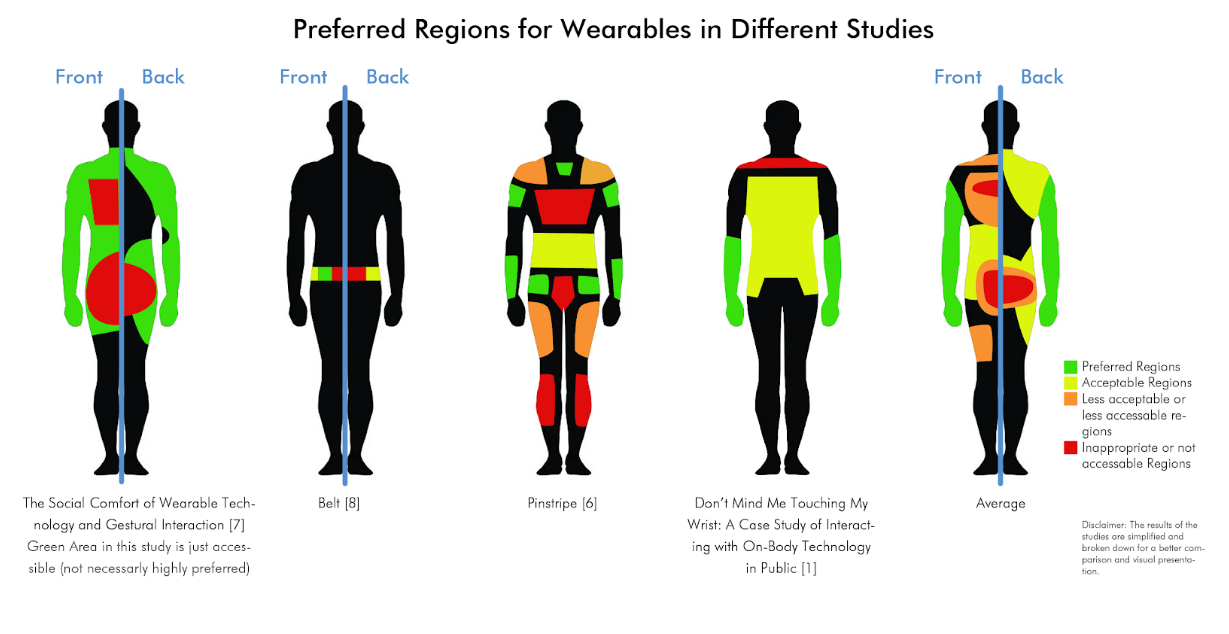
\includegraphics[width=\textwidth]{body-areas.png}
   \caption{Preferred Regions for Wearables in Different Studies Comparison \protect\cite{touch-wrist,pinstripe,social-comfort,belt,simpleskin}}
   \label{fig:body}
 \end{figure*}

 The single most prominent factor mentioned in the respective research projects, besides the type of gesture, was the body region where the Wearable was placed. The figure above shows the preferred regions in the individual studies. When comparing the researches there are two main observations to be made. First there is a strict aversion against socially suggestive regions for Wearables. These regions include genitalia, the bottom and, especially when asking female subjects, the upper torso area, including the sternum and collarbone.
 Second the all around preferred area for Wearable seems to be the forearm and wrist region - especially of the non dominant hand. \cite{touch-wrist,pinstripe,social-comfort,belt} %[1,6,7,8]
 This may be due to the fact that interaction with technologies on these body regions is already established and accepted in society through other devices such as watches and fitness bracelets. However, these body regions are also easy to reach and offer sufficient space for various gestures, which makes these body regions very suitable for body-worn controllers in the future as well.
\section{Outlook on social acceptability of wearables in the future}
Outlook on social acceptability of Wearables in the future

When looking into the future of Wearables one of the most interesting parts is the social acceptability. Since physical comfort, accessibility, and usability are for the most part figured out \cite{social-comfort}.
One, if not the most, important part of social acceptability are the performed gestures. Currently there is always a tradeoff which needs to be balanced when designing gestures, which are meant to be used in public situations. On one hand natural gestures are inherently more unobtrusive and socially acceptable. On the other hand these gestures are far more difficult to track and evaluate precisely, since they are easily confusable with everyday gestures that were not meant to be an input \cite{social-comfort}.
One approach to solve this problem is improving on better technology and tracking to avoid both confusing inputs and social discomfort at the same time. Another approach could be focussed around the social vocabulary more than around the gestures themselves.
``Because there does not currently exist a standard ‘vocabulary’ of gesture, it is correspondingly more difficult for viewers to match a perceived gesture with a previously-understood meaning.'' \cite[p. 4160]{social-comfort} %page 4160
Looking at this quote the other solution seems obvious. With the further adaptation of a novel technology there comes a better understanding of the gestures and finally a new social vocabulary regarding it. There were similar developments when the bluetooth headset \cite{social-comfort} or the Sony Walkman \cite{touch-wrist} was established.
In conclusion, the social acceptance of body-worn controllers can be increased through further developments and by bringing them more and more in contact with the public.

% \section{Second section in another file}
Even if the file is different, using the
\begin{verbatim}
  \section{Second section in another file}
Even if the file is different, using the
\begin{verbatim}
  \section{Second section in another file}
Even if the file is different, using the
\begin{verbatim}
  \include{anotherSection}
\end{verbatim}
we can add the text in the main file.

\end{verbatim}
we can add the text in the main file.

\end{verbatim}
we can add the text in the main file.

\bibliographystyle{SIGCHI-Reference-Format}
\bibliography{biblio.bib}

\end{document}

%%% Local Variables:
%%% mode: latex
%%% TeX-master: t
%%% End:
